\documentclass{tpk4170report}

\title{Title of Report}
\author{Author(s)}

\usepackage{blindtext}

\addbibresource{references.bib} 

\begin{document}

\maketitle

\frontmatter

\chapter*{Preface}

\tableofcontents
\listoffigures
\listoftables

\mainmatter








\chapter{Introduction}
\label{chap:Introduction}

\blindmathtrue
\blindtext

This is a citation~\cite{McCarthy2011}. \blindtext

See Table~\ref{table:floating-table} for a floating table and
\eqref{eq:equation-example} for an equation.
\begin{align}
  \label{eq:equation-example}
  y = ax + b 
    = cz + d 
\end{align}

\begin{table}
  \centering
  \begin{tabular}{l|lll}
    a& b& c &d \\
    \hline
    a& b& c &d \\
    a& b& c &d \\
    a& b& c &d
  \end{tabular}
  \caption{This is a floating table}
  \label{table:floating-table}
\end{table}




\chapter{Forward Kinematics - Task 1}
Denavit-Hartenberg (DH) is a convention broadly used in robotics. It was introduced in order to standardize the attachmemt of cordinate frames to robots. A robot can be seen as a kinematic chain of rigid bodies. These rigid bodies are called links and are connected with joints. A robot arm is represenetd by a kinematic chain which is a concatenation of several links and joints. If one object is manipulated by one robot the system is called open kinematic chain. If several robots manipulate one object simultanously the system is called closed kinematic chain. In this task we will focus on open chain robots. Forward kinematics is a way of of calculating the end effector pose based on the joint parameters. The relation from the end effector to the base is done by attaching one frame to the end effector and one to the base of the robot. The relation between those two frames is then determined by the homogenious transformation matrix \(T_{E}^{B}\). To make things easier a frame can be attached to each link and then the relation between each consecutive frame can be calculated by \(T_{i+1}^{i}\). Concatenating all these homogenious Transformations and building their dot product determines the homogenious Transformation from the robot base to end effector: 
\begin{equation}
  T_{E}^{B} = T_{0}^{1}*T_{1}^{2}* ... *T_{i-1}^{i}
  \label{eqn:recursive_expression_homogenious_transformation}
\end{equation}
Denavit-Hartenberg (DH) is a convention which standardizes the attachmemt of cordinate frames to a robot. It is a convention broadly used in the community which makes the application of the recursive formula in \ref{eqn:recursive_expression_homogenious_transformation} more intuitive. The DH convention provides rules how to attach the frames to the link. In general the result should be the same if the frames are attached differently to the links as long as every link is considered. In the DH convention four different parameters afe used in order to attach frames to the robot links. The frame of the link i+1 is determined based on the frame of the link i. The placement of a frame is visulaized in \ref{fig:Denavit_Hartenberg_Konvention_Rules}. The followinfg consecutive rules are applied:

\begin{itemize}
  \item[1] \(z_{i}\) alligns with the rotational axis of joint i+1
  \item[2] \(O_{i}\) is placed at the intersetion of \(z_{i}\) and the common normal of \(z_{i-1}\) and \(z_{i}\) 
  \item[3] \(O_{i'}\) is placed at the intersetion of \(z_{i-1}\) and the common normal of \(z_{i-1}\) and \(z_{i}\)
  \item[4] \(x_{i}\) alligns with the common normal of \(z_{i-1}\) and \(z_{i}\) pointing away from \(O_{i'}\)
  \item[5] \(y_{i}\) is chosen according to the right hand rule
  \end{itemize}
\begin{figure}
  \centering
  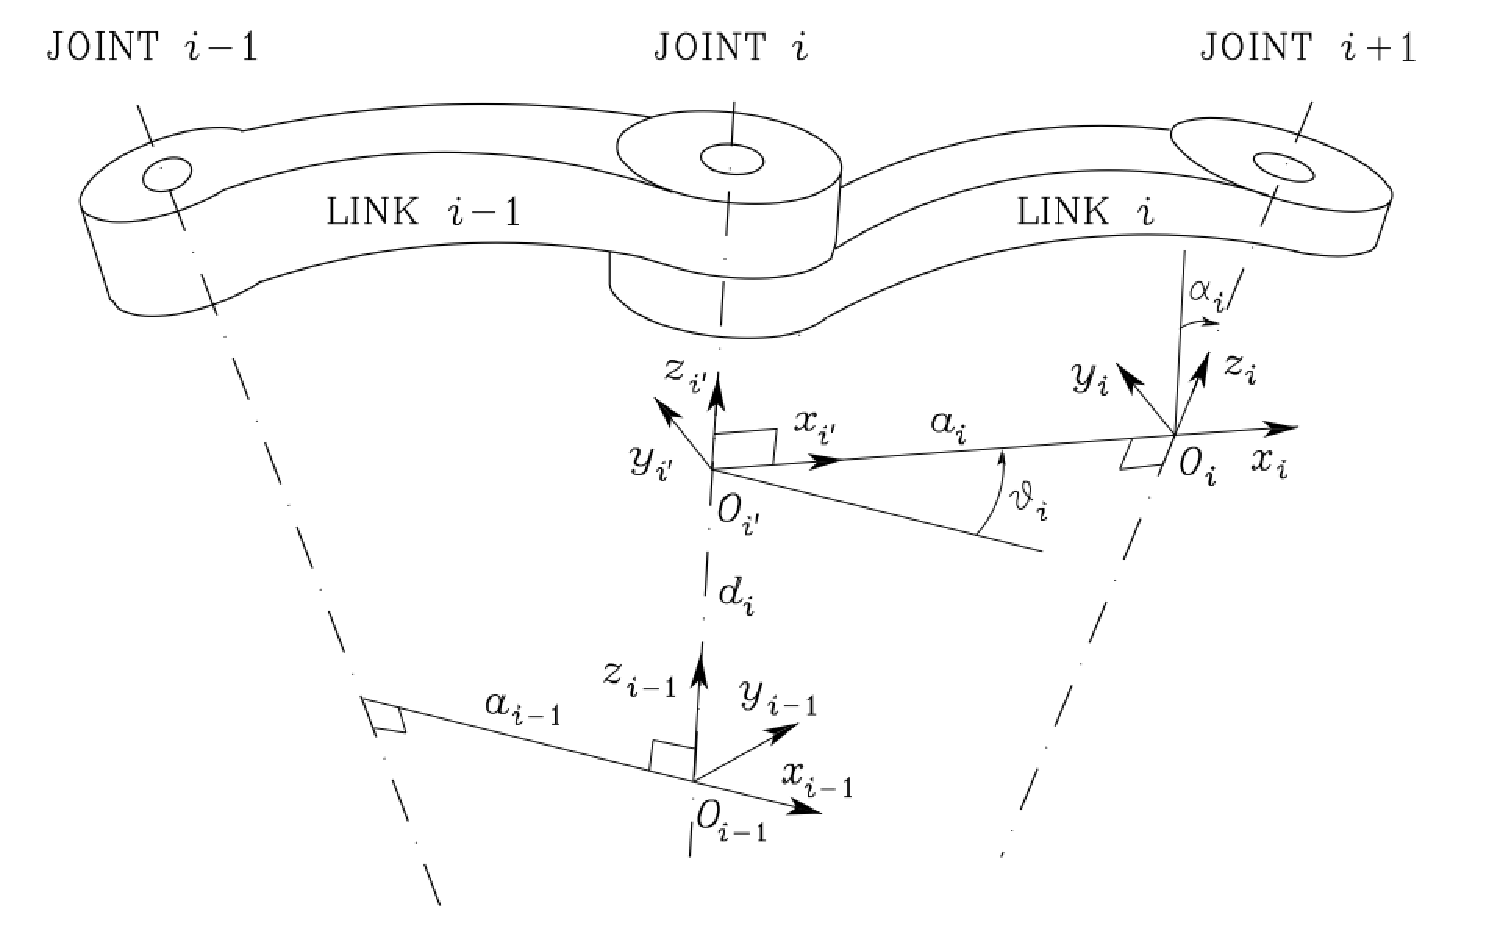
\includegraphics[width=0.8\textwidth]{assets/Denavit_Hartenberg_Convention_Rules.pdf} 
  \caption{Denavit Hartenberg convention rules}
  \label{fig:Denavit_Hartenberg_Konvention_Rules}
\end{figure}

The DH convention does not define enough rules to make sure that there is just one uniquie solution. 

\begin{itemize}
  \item[1] There is no frame i-1 for frame 0 we can not define \(O_{i}\) and \(x_{0}\):  \(O_{i}\) and \(x_{0}\) can be defined arbitrarily.
  \item[2] There is no joint i+1 when defining frame n we can not define \(z_{i}\): \(z_{i}\) is defined parallel to \(z_{i-1}\) . 
\end{itemize}  Usually there are some ways of defining those two parameters which make applying the convention easier.

There are some special cases which also do not allow a unique definition of frames:
\begin{itemize}
  \item[1] \(z_{i+1}\) and \(z_{i}\) are parallel: \(O_{i}\) and \(x_{i}\) can be selected arbitrarily.
  \item[2] \(z_{i+1}\) and \(z_{i}\) are parallel: \(O_{i}\) and \(x_{i}\) can be selected arbitrarily.
  \item[3] joint i is prismatic: \(x_{i-1}\) can be selected arbitrarily.
\end{itemize}

The DH convention makes finding the homogenious transformations especially convenient. After establishing the frames at each joint the four DH parameters can be identified. 

\begin{itemize}
  \item[\(a_{i}\)]: distance between \(O_{i}\) and \(O_{i'}\) 
  \item[\(d_{i}\)]: distance between \(O_{i'}\) and \(O_{i-1}\) along \(z_{i-1}\)
  \item[\(\alpha_{i}\)]: angle between \(z_{i-1}\) and \(z_{i}\) about \(x_{i}\)
  \item[\(\vartheta{i}\)]:  angle between \(x_{i-1}\) and \(x_{i}\) about \(z_{i-1}\)
\end{itemize}

The paramters \(a_{i}\) and \(\alpha_{i}\) are constantg and just depend on the geometry of the link i. Non constant is the parameter \(d_{i}\) if joint i is prismatic and the parameter \(\vartheta{i}\) if joint i is rotational.

Having the four parameters \(a_{i}\), \(d_{i}\), \(\alpha_{i}\), \(\vartheta_{i}\)one can write down the homogenious transformations T immediatelly: 

\begin{equation}
  T_{i}^{i-1}= 
  \begin{bmatrix}
    c_{\vartheta_{i}} & -s_{\vartheta_{i}}c_{\alpha_{i}} &  s_{\vartheta_{i}}s_{\alpha{i}} & a_{i}c_{\vartheta_{i}} \\
    s_{\vartheta_{i}} & c_{\vartheta_{i}}c_{\alpha{i}} & -c_{\vartheta_{i}}s_{\alpha{i}} & a_{i}s_{\vartheta_{i}} \\
    0 & s_{\alpha{i}} & c_{\alpha{i}} & d_{i} \\
    0 & 0 & 0 & 1
  \end{bmatrix}
  \label{eqn:Transformation_Denavit_Hartenberg}
\end{equation}
\chapter{Here Comes Chapter 2}

\Blindtext

\begin{figure}
  \centering
  
\includegraphics[width=0.5\textwidth]{hovedlogo} 
  \caption{NTNU logo}
  \label{fig:logo2}
\end{figure}

\section{Title of section 2}








\chapter{Here Comes Chapter 3}

\Blindtext

\begin{figure}
  \centering
  
\includegraphics[width=0.5\textwidth]{hovedlogo} 
  \caption{NTNU logo}
  \label{fig:logo}
\end{figure}





\chapter{Conclusion}

\blindtext[4]



\printbibliography[title=References]

\appendix
\chapter{Name of Appendix} 

\section{This is a section}

\end{document}